\clearpage
\section{Supplemental Information}

\begin{algorithm}[th]
        \begin{algorithmic}[1]
        \label{alg:alg1}
        \caption{\name{}'s Training Algorithm}
        % \textbf{Input} Dataset $D$
        \STATE Train the ATENA~\S{5.2} on given dataset $D$
        \STATE Generate sequences $O$ using ATENA
        \STATE Train a $BTM$ model $\phi$ with $K$ topics on $O$
        \STATE Create sample set $A=\{a_1,a_2,...,a_i\}_{i=1}^n$
        \STATE Initialise A2C model
        \FOR{$i = 1,...,episodes$}
            \STATE Initialize the state space $s_t$ as in (\ref{eq:state_space}) with zeroes
            \FOR{$t = 1,...,l$}                    
                    \STATE Generate a query $q_t$ from the simulator
                    \STATE Take action $a_t$ for the given $s_t$
                    \STATE Update $s_t$ with latest query $q_t$, display vectors $v_t$, latency $C_t$ and current intent as $\phi(Q_t)$
            \ENDFOR
            \STATE Calculate Individual rewards using~\S{4.3}.
            \STATE Calculate the total reward $R_t$
            \STATE Calculate $J_R(\pi) = \mathbb{E}_{a_t \sim \pi_\theta}[R_t]$
            \STATE Compute loss functions $\mathbb{L}(\theta)$ for policy network
            \STATE Compute $\mathbb{L}(\omega)$ for value network
            \STATE Update A2C model
        \ENDFOR
        \end{algorithmic}
    \end{algorithm}

\subsection{Formal Problem Formulation}
\label{sec:problem}
%
%\sm{Please review. Does this problem formulation make sense or does it becomes confusing or conflicting}


%
%\tong{Is $D$ the variable $A$ in Section 4.1?}
%\sm{Yes}
Let $D_0$ be the full data target for EDA.
Let $D'$ = $\{D_i\}_{i=1}^n$ be $n$ subsamples created from $D$ and $|D_i| < |D_0|$ for $i \in [1, n]$ where $|.|$ denotes size (\# of rows). 
Let an $l$ length EDA session $e=\langle \{q_j(D_i), v_j(D_i)\}_{j=1}^l | i \in [1,n]\rangle$ be comprised of an alternating sequence of queries $q_j(.)$ and corresponding results/visual output $v_j(.)$ performed on data $D_i$. 
Note $D$ is the variable $A$ in Section 4.1 and line 4 of Algorithm 1.
%

Let $I$ be the set of implicit intents embedded in the distribution of all $e$, the EDA sessions.
%\sg{What is e here?}\sm{e is an EDA sequence/session}
%
Let $I^{D_0}$ be original distribution of the intents $P(I|D_0)$, i.e. when all EDA was done using full data $D_0$.
Let $I^{D'}$ be the distribution $P(I|D')$, i.e., EDA is approximated using only subsamples.
Our goal is to find optimal subsample $D_i, i \in [1,n]$ for each step of the EDA $\{q_j(.), v_j(.)\}$ such that $Div(I^{D_0}||I^{D'})$ is minimized with $I$ as the support.
%

We define $Div(I^{D_0}||I^{D'})$ as the \textbf{intent-divergence} between the EDA performed using full data and approximate EDA using only subsampled data. 

\subsection{Discussion: Intent-divergence vs. intent-shift}
\label{app:discussion_intent_shift}

Please note, in this paper we address the problem of \textit{intent-divergence} where the users' have a set of consistent implicit objectives/intents during the EDA. 
While \name{} deliberately introduces a bias towards a set of intents inferred from historical analysis sequences, this is justified as real expert users often follow some standard exploration strategies and look for similar types of insights even on new datasets as observed by multiple prior works~\cite{atena2020sigmod, jain2016sqlshare, milo2018next} and do not perform random explorations.
However, if such implicit objectives suddenly change causing an \textit{intent-shift}, then \name{}'s current design would not be able to detect that. 
In this paper, it is assumed that there is limited \textit{intent-shift} (\emph{i.e.}, change of user's core intent characteristics). 
%While in this paper we are the first to address how to prevent intent-divergence (approximation errors misleads users to a different intent), 
This assumption is widely adopted in other interactive applications \cite{liu2018dialogue,guo2018dialog,tan2019drill}, although it is interesting to address the intent-shift \cite{xie2021tiage,arnold2019sector}. As the first work on approximate exploratory data analysis in the interactive setting, we leave addressing \textit{intent-shift} as future work.


\begin{figure*}[!t]
\centering
\begin{minipage}[t]{0.57\textwidth}
\vspace{0pt}
\begin{subfigure}{.5\textwidth}
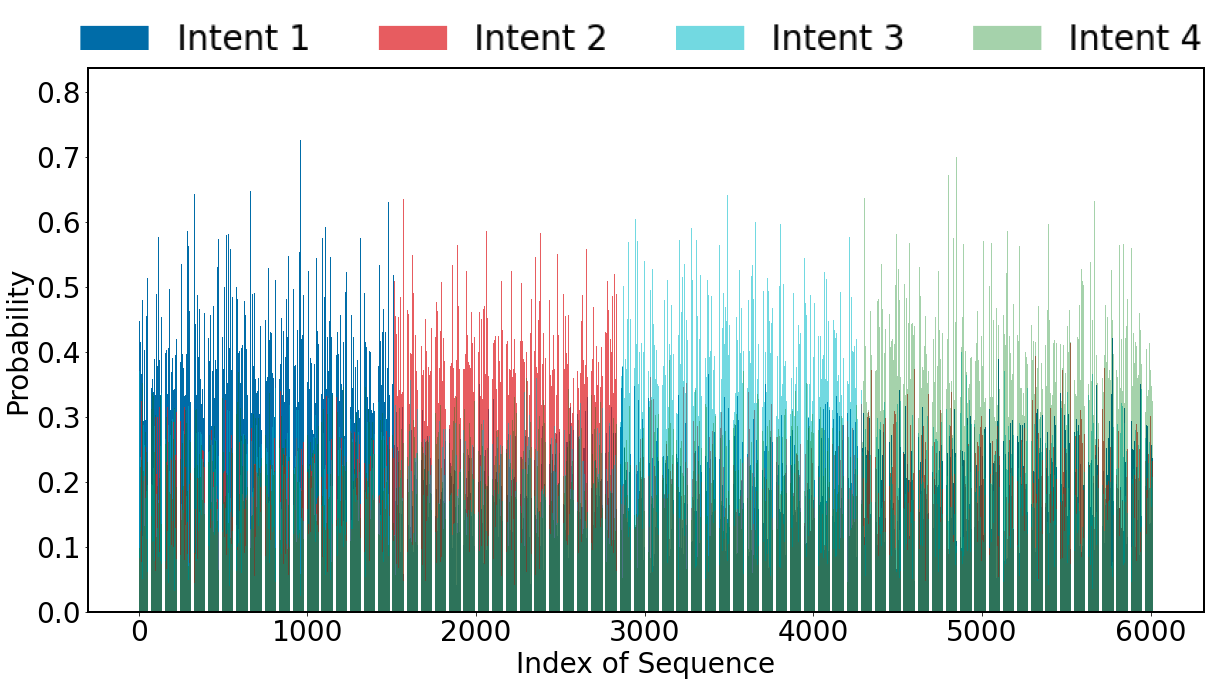
\includegraphics[width=1.0\linewidth]{LaTeX/figures/intentcl1.png}
\caption{EDA on Flights Dataset}
\end{subfigure}
\begin{subfigure}{.5\textwidth}
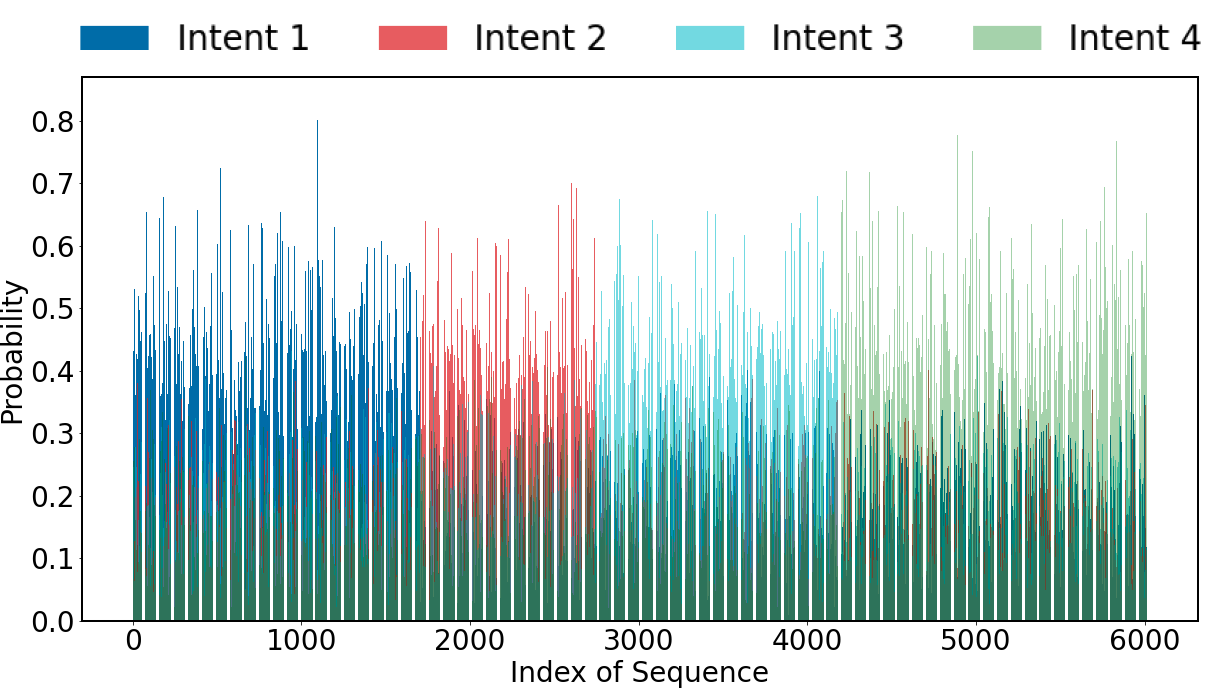
\includegraphics[width=1.0\linewidth]{LaTeX/figures/intentcl2.png}
\caption{EDA on Housing Dataset}
\end{subfigure}
     \caption{The probability distribution of query sequences for each of the identified $k=4$ intents. The sequences are grouped together intent-wise. This graph illustrates the distinguishable definitions of intents through their probability distributions. Since trend on Income dataset is similar, we omit the details.}
     \label{fig:intent_cluster}
\end{minipage}
%\hfill
\hspace{0.05\textwidth}
\begin{minipage}[t]{0.37\textwidth}
\vspace{0pt}
\begin{subfigure}{1.0\textwidth}
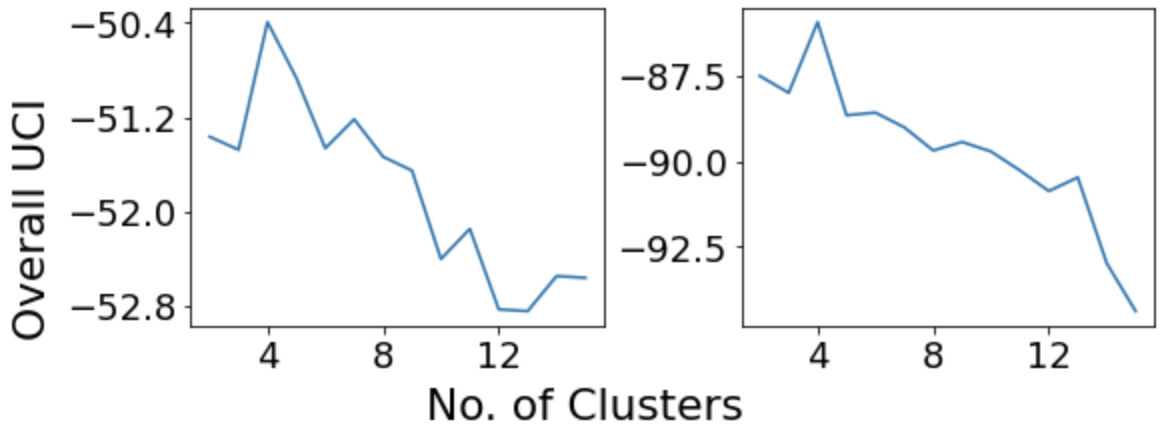
\includegraphics[width=1.0\linewidth]{LaTeX/figures/uci_plot_new.png}
%\caption{UCI measure for different number of cluster}
\end{subfigure}
\caption{UCI measure for different number of clusters (Left: Flights, Right: Housing data). Overall UCI is the highest when $K=4$ for both. Since trend on Income dataset is similar, we omit the details.}
     \label{fig:intent_clusters}
\end{minipage}
%\begin{minipage}[t]{0.2\textwidth}
%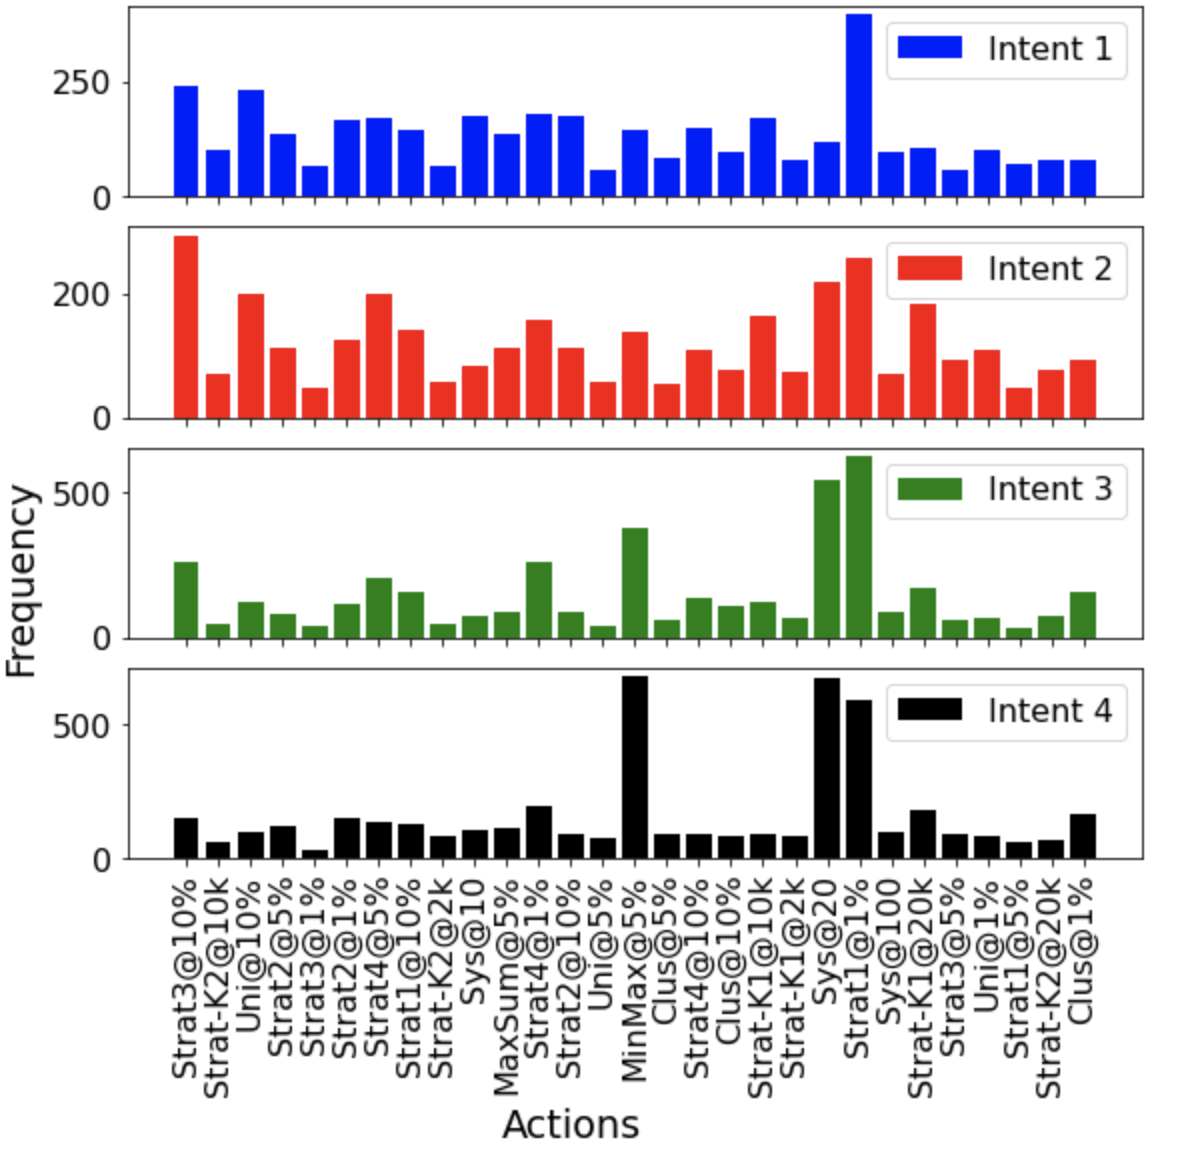
\includegraphics[width=\linewidth]{LaTeX/figures/intent_actions2.png}
%     \caption{Frequency of different actions taken by \name{} for different intents.}
%     \label{fig:action_usage}
%\end{minipage}
\vspace{-0.5em}
\end{figure*}

\subsection{Discussions: Design and Deployment}
\label{app:discussion}

\noindent\textbf{RL vs. Greedy Solutions.}

Simple greedy solutions would not work because because of the following reasons:
(1) It is impossible to calculate an approximation error when a query is run against each of the samples, unless we also run it against the original data at run-time (which defeats the purpose of using samples), 
(2) Even if we calculate an estimate of the approximation error, choosing the sampling strategy that minimizes error for each query may not be optimal because a less-accurate strategy might be of significantly lesser size, but still contain enough information that would preserve the high-level signal in the results (e.g. a bar being substantially higher than the rest) and would not lead to a wrong decisions by the analyst while choosing subsequent queries.

\noindent\textbf{Deployment Aspects.}

Significant history of EDA analysis sequence gets generated for data analysis usecases related to e-commerce, web/mobile analytics or digital marketing setting, where several analysts repeatedly explore the data to constantly understand different aspects of customer behavior. 
%At certain intervals, more recent data is ingested in batch and appended with the existing data causing the data-size to become significantly larger over time. 
%
In production scenario, different samples  are periodically regenerated in an offline manner as new batch of data of significant size is ingested. 
However, according to our understanding from experts, the EDA analysis patterns and intents for a particular dataset remains same over time (also refer to \S~\ref{app:discussion_intent_shift}).
Since, the overall characteristics of intents of the analysts do not change, \name{}'s learning about the effectiveness of different samples under different contexts does not get significantly affected if the overall statistical characteristics of the freshly ingested data is consistent with the old one.
However, if the statistical characteristics change, then \name{} is retrained with new samples in the background and after convergence the old model is replaced. 



\subsection{More Ablation Study Results}

\begin{table}[th]
\tiny

\label{table:ablation_delta}
\begin{tabular}{|l|l|l|llll|}
\hline
\multicolumn{1}{|c|}{\multirow{2}{*}{\begin{tabular}[c]{@{}c@{}}Model \\ Parameter\end{tabular}}} & \multicolumn{1}{c|}{\multirow{2}{*}{Relative ED}} & \multicolumn{1}{c|}{\multirow{2}{*}{\begin{tabular}[c]{@{}c@{}}Latency \\ Reduction\end{tabular}}} & \multicolumn{4}{c|}{\begin{tabular}[c]{@{}c@{}}Mean Overall\\  Recall\end{tabular}}                                           \\ \cline{4-7} 
\multicolumn{1}{|c|}{}                                                                            & \multicolumn{1}{c|}{}                             & \multicolumn{1}{c|}{}                                                                              & \multicolumn{1}{c|}{Intent 1} & \multicolumn{1}{c|}{Intent 2} & \multicolumn{1}{c|}{Intent 3} & \multicolumn{1}{c|}{Intent 4} \\ \hline
$\delta =1$                                                                                         & 1                                                 & 0.89                                                                                               & \multicolumn{1}{l|}{0.32}     & \multicolumn{1}{l|}{0.74}     & \multicolumn{1}{l|}{0.29}     & 0.68                          \\ \hline
$\delta = 0$                                                                                        & 1.2                                               & 0.90                                                                                               & \multicolumn{1}{l|}{0.31}     & \multicolumn{1}{l|}{0.61}     & \multicolumn{1}{l|}{0.3}      & 0.42                          \\ \hline
\end{tabular}
\caption{Ablation study: Variation of $\delta$ in $R_{intent} = R_{dis} + \delta*R_{topic}$ (Ref. \S~\ref{sec:reward}).}
\label{tbl:ablation_delta}
\end{table}

Recall in \S~\ref{sec:reward}, we use full intent reward as: $R_{intent} = R_{dis} + \delta*R_{topic}$.
We do an ablation study on this $\delta$ and show in Table~\ref{tbl:ablation_delta}.
We observe that both components of our reward are important. Setting $\delta=0$ increases our relative distance between distributions. Although it reduces the latency, the gain is small. We also see that for various intents, our recall decreases significantly for Intent 2 and Intent 4. This is because setting $\delta=0$ removes the component that matches intent of the original sequence with the generated.

\begin{table}[]
\scalebox{0.8}{
\begin{tabular}{|l|l|}
\hline
No. of Intents & \begin{tabular}[c]{@{}l@{}}Relative  ED\end{tabular} \\ \hline
4              & 1                                                     \\ \hline
6              & 2.98                                                  \\ \hline
8              & 5.84                                                  \\ \hline
10             & 7.41                                                  \\ \hline
\end{tabular}
}
\caption{Ablation study: Variation of K or \# of intents (Ref ~\S{\ref{sec:intent_identification}})}
\label{tbl:ablation_K_intent}
\end{table}

In Table~\ref{tbl:ablation_K_intent} we show ablation study for Flights dataset on number of intents used ($K$) (Ref. ~\S{\ref{sec:intent_identification}}) and how Euclidean Distance (ED) from ideal changes (increase in ED is worse) relative to the distance for number of intents $K=4.$

% Please add the following required packages to your document preamble:
% \usepackage{multirow}


\subsection{Intent Identification Results} 
\label{apps:intent_identification}


Figure~\ref{fig:intent_cluster} shows the probability distribution of intents for each of the query sequence and the 4 clusters identified can be clearly observed for Flights and Housing datasets. 
Since trend on Income dataset is similar, we omit the details.
To choose the best value for the number of intents, $K$, we compute the overall UCI score for all $K \in [2,15]$ and choose the best K. As can be seen maximum UCI score is observable at K=4.
%\tong{this sentence and figures may be moved to the appendix?}

\subsection{Model and Implementation Details}
\label{apps:model_implementation}
% \tong{I merged two appendix sections into one section. Please make sure the original referred appendix section ID is still valid in the paper content (i.e., first 9 pages).}
Our approach is based on A2C, an actor critic model for the training of our RL Agent. An actor critic model consists of two parts, an actor (policy network) which takes the state of the agent and outputs the best possible action, whereas the critic (value network) evaluates the action by computing the value function. %These two networks incrementally get better at their roles and the resultant architecture is better than the two methods separately.

%To train our A2C model, we use two separate networks. The policy network is a fully connected neural network and its task is to produce the best action given the agent state. The value network is also a fully connected neural network, and it receives the input as the state of the agent and the action chosen by the policy and outputs the Advantage value. This advantage value is the estimate of how good the chosen action can be in future. The training of both the networks happens separately and it uses gradient ascent to update the weights. The update of weights happen at each step (TD Learning).

To train our model, we generate 10k sequences using the simulator~\cite{atena2020sigmod} and we get 5995 unique sequences for the flights dataset and 6016 sequences for the housing dataset. We use $K=4$ for our experiments. To train the RL agent, for both policy network and value network, we use neural networks consisting of 2 fully-connected layers, with a dimension of 64 each. The activation function used is $\tanh$. The policy model used is MlpPolicy and we set the number of environments to 64. For the A2C model, we set the value function coefficient, $vf_{coef} = 0.25$ and the entropy coefficient, $ent_{coef} = 0.01$. The learning rate used for the model is 0.0007. More details about the algorithm are explained in \S{\ref{app:training}}
 
For the reward calculation, we scale all the rewards between $[-0.5, 0.5]$. For training \name{}, we used $\delta=1, \zeta=1$. To give equal weight to all the reward components, we set the value of $\beta=0.5, \gamma=0.5$. \ref{tab:model-details} shows some details for the trained model.

Tables \ref{tab:flights_samples}, \ref{tab:housing_samples} and \ref{tab:income_samples} show the actual number of rows sampled from each dataset and presents the Effective Sampling Rate (ESR). We create 29 samples for the \textit{Flights dataset} as shown and create 15 samples for each of \textit{Housing dataset} and \textit{Income dataset}.
In Figure~\ref{fig:my_conv} we show the training convergence curves. For evaluation, we choose the model with the best possible reward. The no. of steps for selection of the model is given in Table 7.

\begin{table}[H]
\vspace{0pt}
\scalebox{1}{
\begin{tabular}{|l|l|l|l|}
\hline
Dataset & \begin{tabular}[c]{@{}l@{}}No. of \\ steps\end{tabular} & Time(hr) & Model Size(KiB) \\ \hline
Housing & 36k                                                       & 20.3     & 284       \\ \hline
Flights & 36k                                                       & 15.8     & 363       \\ \hline
Income & 33k                                                       & 16.7     & 312       \\ \hline
\end{tabular}
}
\caption{Training times and model sizes}
\label{tab:model-details}
\end{table}
 
\subsection{Training Algorithm}
\label{app:training}
% \tong{I slightly changed the following algorithm. Please check whether the updated version looks good.}
Algorithm 1 explains the steps we use for training our RL Agent. It takes in the dataset $D$, processes it by creating samples as shown in line 4 and training ATENA simulator on the same as shown in line 1. Then on the generated sequences, a BTM model is trained in line 3. Once this is done, we then start the training of our agent as demonstrated in lines 5-18 of Algorithm 1. We follow episodic training where we calculate rewards at the end of each episode as shown in line 13. Once we calculate the total reward, we compute the loss functions and update both actor (policy) and critic (value) networks as explained in \S{\ref{apps:model_implementation}}. 

\subsection{Qualitative Evaluation}
\label{apps:qualitative_eval}
%\vspace{-0.2em}
%
\begin{figure}[th!]
\begin{minipage}[t]{1.0\columnwidth}
\vspace{0pt}
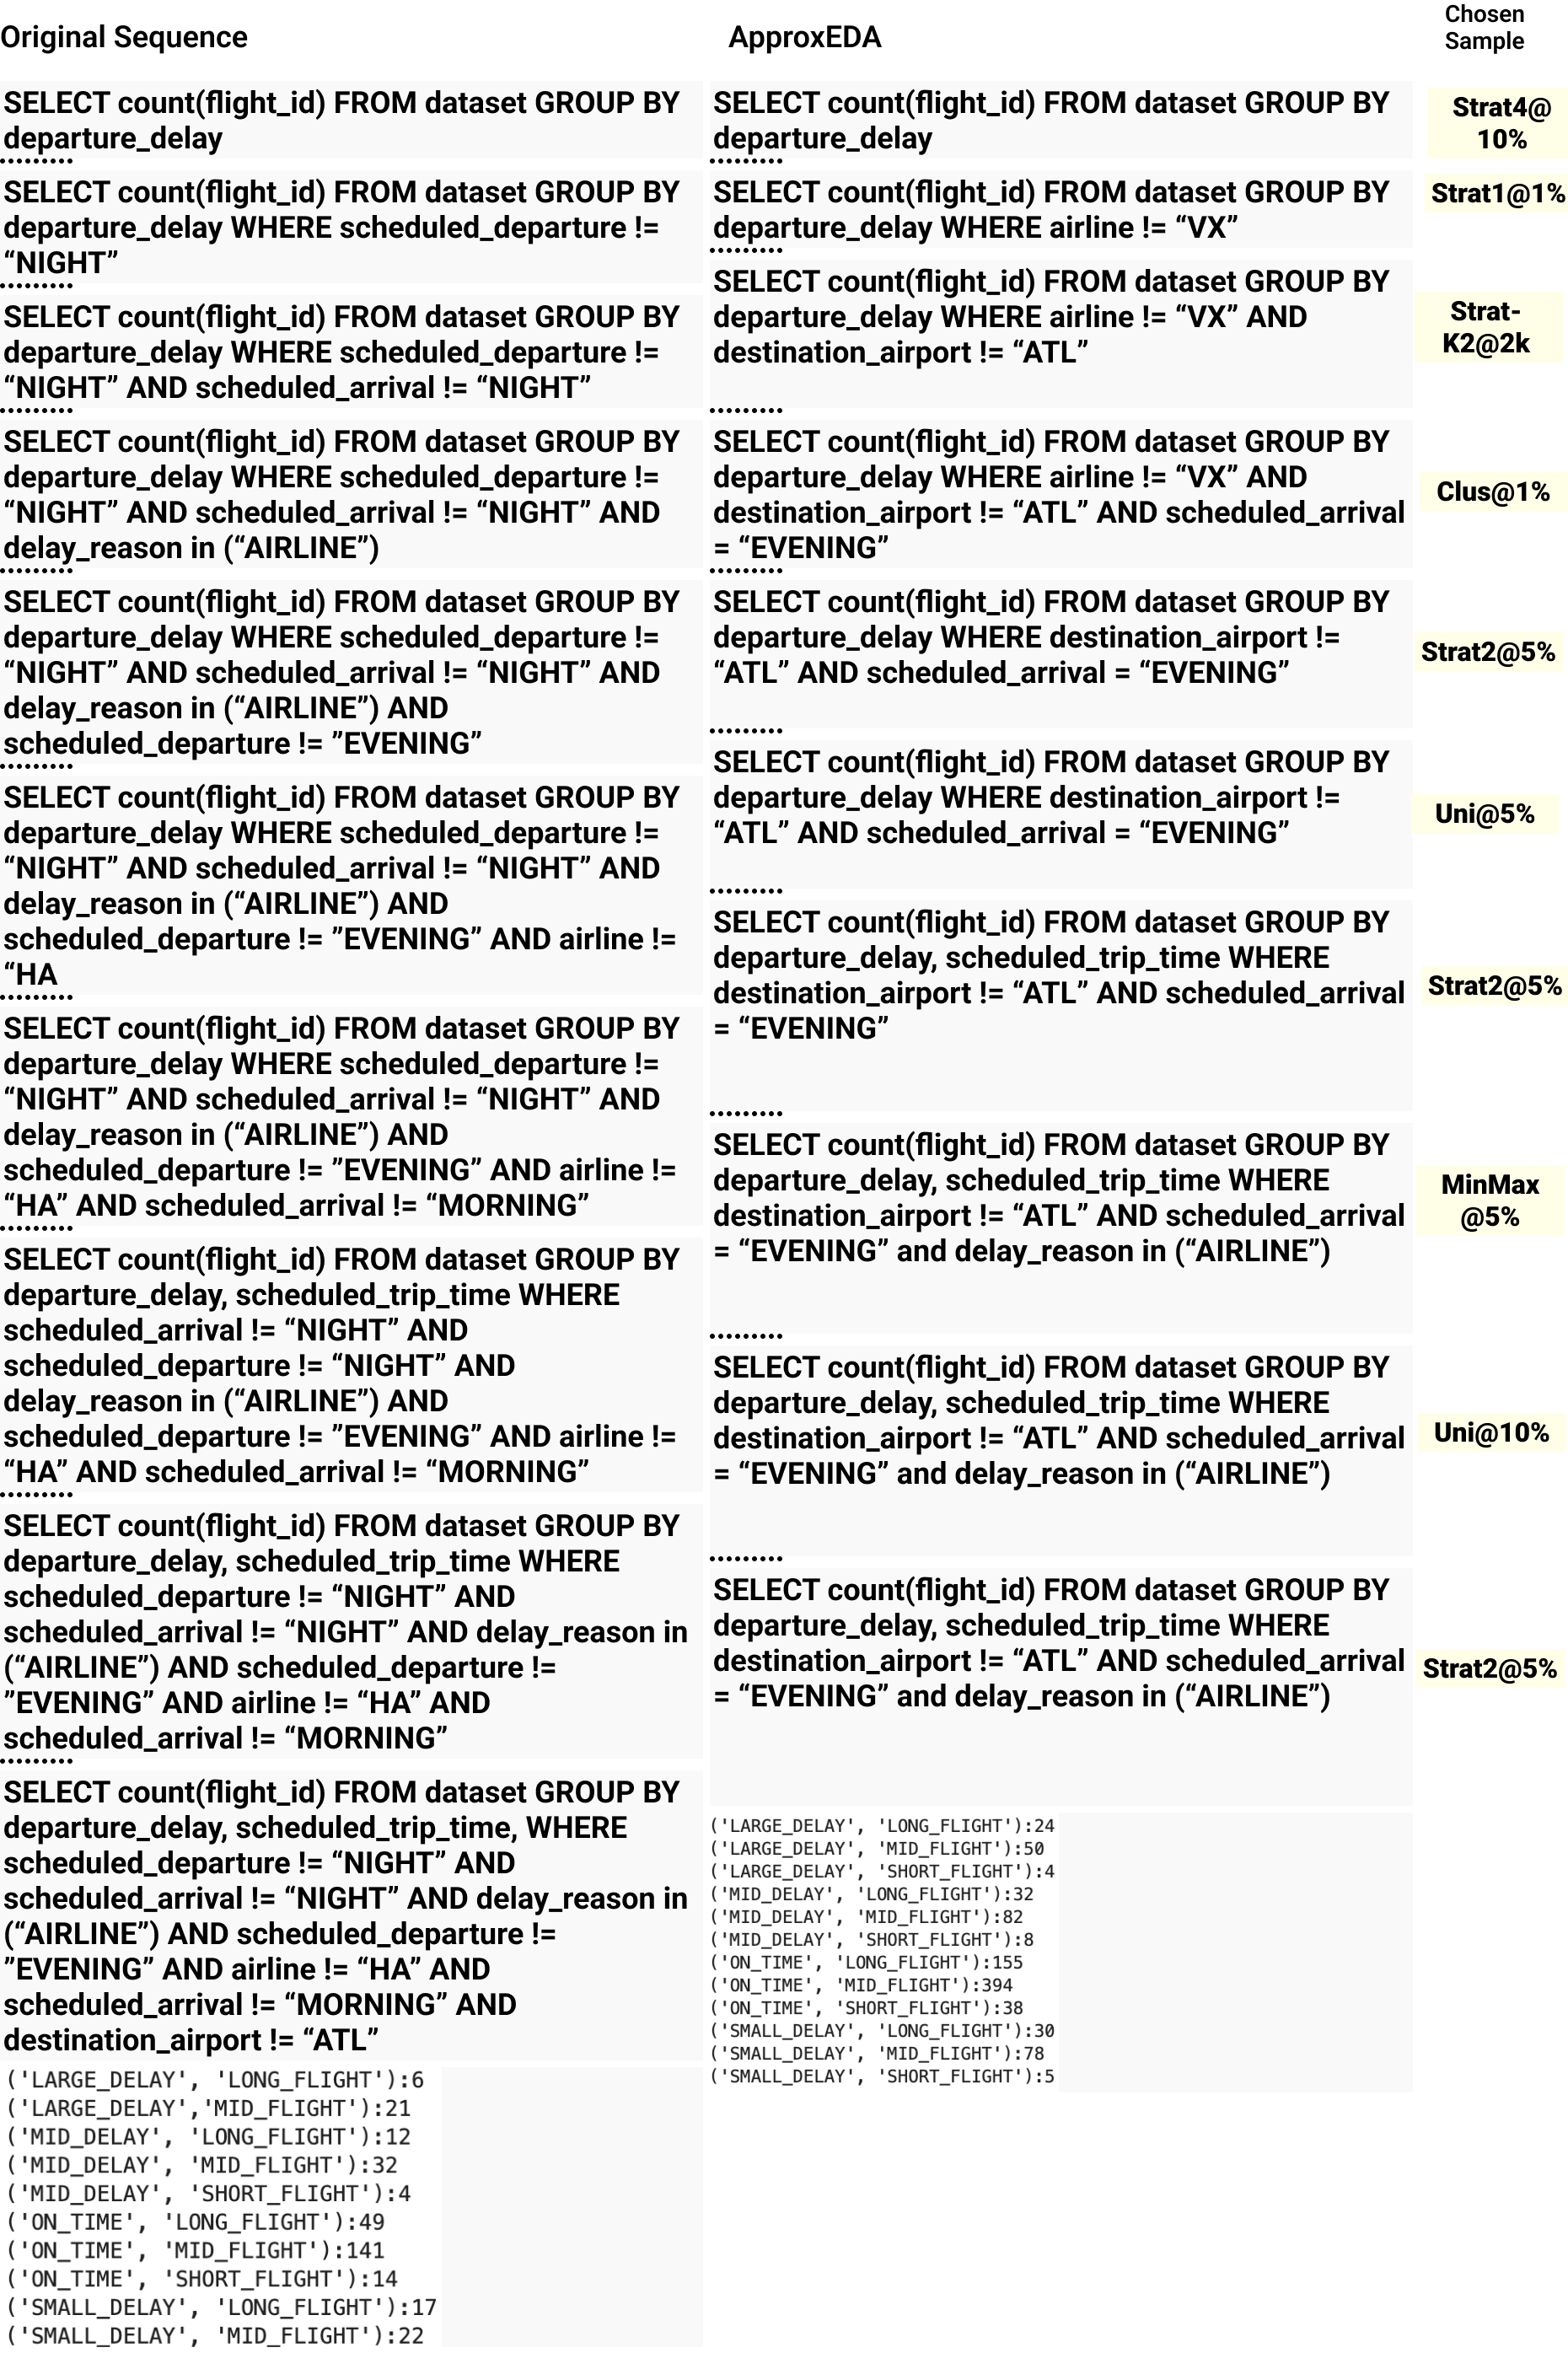
\includegraphics[width=1.0\columnwidth]{LaTeX/figures/appendix_seq.png}
     \caption{%Snapshot of an EDA sequence 
     An example EDA sequence from the logged results,
     showing how \name{} can efficiently preserve the query structure, analysis sequence and final outcome/insight by selecting various different samples (annotations on the right) under the hood to maximize its objective.}
     \label{fig:real}
\end{minipage}
\end{figure}

Figure~\ref{fig:real} we show a real EDA session with \name{}, where it 
selected various different samples (annotations on the right) to maximize its objective. We can see in-spite of it selecting fery frugal samples at various points (e.g. Clus@1\%, Uni@5\% etc.), \name{} can mostly preserve the query structure, analysis sequence and final outcome/insight. 
In Figure~\ref{fig:action_usage} we show the variation of \name{}'s choice of different actions (selection of samples) for 4 different intents identified for the Flights data across all the held out sequences.
We found that certain samples (e.g. MaxMin@5\%, Sys@20\%, Strat1@1\%) were predominantly chosen for certain intents (e.g. \#4). Intuition is that such samples can preserve representations of smaller groups better, which is necessary for that intent preservation.


%Then it will interact with the users' EDA sessions almost transparently. 


\subsection{Additional Results}
\label{app:add_res}
Similar to \ref{sec:eval_insight}, we also compute the recall for all the results instead of just 5. We show the results in \ref{fig:recall}. Even in the case of the whole recall \name{} seems to do better than the baselines.

\begin{figure}[!t]
\centering
\begin{minipage}[t]{0.495\columnwidth}
\vspace{0pt}
% \begin{table}[]
\scalebox{0.65}{
\begin{tabular}{|l|l|l|}
\hline
\begin{tabular}[c]{@{}l@{}}Sampling \\ Strategy\end{tabular} & \begin{tabular}[c]{@{}l@{}}No. of \\ Rows\end{tabular} & \begin{tabular}[c]{@{}l@{}}Effective\\  SR\end{tabular} \\ \hline
Uni@1\%                                                      & 5232                                                   & 0.01                                                    \\ \hline
Uni@5\%                                                      & 26155                                                  & 0.05                                                    \\ \hline
Uni@10\%                                                     & 52312                                                  & 0.1                                                     \\ \hline
Sys@100                                                      & 5231                                                   & 0.01                                                    \\ \hline
Sys@20                                                       & 26154                                                  & 0.05                                                    \\ \hline
Sys@10                                                       & 52311                                                  & 0.1                                                     \\ \hline
Clus@1\%                                                     & 5230                                                   & 0.01                                                    \\ \hline
Clus@5\%                                                     & 26154                                                  & 0.05                                                    \\ \hline
Clus@10\%                                                    & 52306                                                  & 0.1                                                     \\ \hline
MinMax@5\%                                                   & 27202                                                  & 0.052                                                   \\ \hline
MaxSum@5\%                                                   & 25109                                                  & 0.048                                                   \\ \hline
KStrat1@2k                                                   & 14124                                                  & 0.027                                                   \\ \hline
KStrat1@10k                                                  & 28771                                                  & 0.055                                                   \\ \hline
KStrat1@20k                                                  & 57542                                                  & 0.11                                                    \\ \hline
KStrat2@2k                                                   & 9416                                                   & 0.018                                                   \\ \hline
KStrat2@10k                                                  & 25125                                                  & 0.048                                                   \\ \hline
KStrat2@20k                                                  & 47080                                                  & 0.09                                                    \\ \hline
Strat1@1\%                                                   & 5220                                                   & 0.01                                                    \\ \hline
Strat1@5\%                                                   & 26146                                                  & 0.05                                                    \\ \hline
Strat1@10\%                                                  & 52375                                                  & 0.1                                                     \\ \hline
Strat2@1\%                                                   & 5232                                                   & 0.01                                                    \\ \hline
Strat2@5\%                                                   & 26148                                                  & 0.05                                                    \\ \hline
Strat2@10\%                                                  & 52320                                                  & 0.1                                                     \\ \hline
Strat3@1\%                                                   & 5240                                                   & 0.01                                                    \\ \hline
Strat3@5\%                                                   & 26150                                                  & 0.05                                                    \\ \hline
Strat3@10\%                                                  & 52315                                                  & 0.1                                                     \\ \hline
Strat4@1\%                                                   & 5235                                                   & 0.01                                                    \\ \hline
Strat4@5\%                                                   & 26149                                                  & 0.05                                                    \\ \hline
Strat4@10\%                                                  & 52321                                                  & 0.1                                                     \\ \hline
\end{tabular}
}
\captionof{table}{Details of Samples generated on Flights Dataset}
\label{tab:flights_samples}
\end{minipage}%
\hfill
\begin{minipage}[t]{0.495\columnwidth}
\vspace{0pt}
\begin{minipage}[t]{1.0\columnwidth}
\begin{minipage}[t]{1.0\columnwidth}
\vspace{0pt}
\scalebox{0.65}{
\begin{tabular}{|l|l|l|}
\hline
\begin{tabular}[c]{@{}l@{}}Sampling \\ Strategy\end{tabular} & \begin{tabular}[c]{@{}l@{}}No. of \\ Rows\end{tabular} & \begin{tabular}[c]{@{}l@{}}Effective\\  SR\end{tabular} \\ \hline
Uni@1\%                                                      & 3242                                                   & 0.01                                                    \\ \hline
Uni@5\%                                                      & 16210                                                  & 0.05                                                    \\ \hline
Uni@10\%                                                     & 32419                                                  & 0.1                                                     \\ \hline
Sys@100                                                      & 3241                                                   & 0.01                                                    \\ \hline
Sys@20                                                       & 16209                                                  & 0.05                                                    \\ \hline
Sys@10                                                       & 32419                                                  & 0.1                                                     \\ \hline
Strat1@1\%                                                   & 3246                                                   & 0.01                                                    \\ \hline
Strat1@5\%                                                   & 16225                                                  & 0.05                                                    \\ \hline
Strat1@10\%                                                  & 32425                                                  & 0.1                                                     \\ \hline
Strat2@1\%                                                   & 3238                                                   & 0.01                                                    \\ \hline
Strat2@5\%                                                   & 16215                                                  & 0.05                                                    \\ \hline
Strat2@10\%                                                  & 32426                                                  & 0.1                                                     \\ \hline
Strat3@1\%                                                   & 3240                                                   & 0.01                                                    \\ \hline
Strat3@5\%                                                   & 16208                                                  & 0.05                                                    \\ \hline
Strat3@10\%                                                  & 32420                                                  & 0.1                                                     \\ \hline
Strat4@1\%                                                   & 3248                                                   & 0.01                                                    \\ \hline
Strat4@5\%                                                   & 16206                                                  & 0.05                                                    \\ \hline
Strat4@10\%                                                  & 32425                                                  & 0.1                                                     \\ \hline
\end{tabular}
}

\captionof{table}{Details of Samples generated on Housing Dataset}
\label{tab:housing_samples}
\end{minipage}
\begin{minipage}[t]{1.0\columnwidth}
\scalebox{0.65}{
\begin{tabular}{|l|l|l|}
\hline
\begin{tabular}[c]{@{}l@{}}Sampling \\ Strategy\end{tabular} & \begin{tabular}[c]{@{}l@{}}No. of \\ Rows\end{tabular} & \begin{tabular}[c]{@{}l@{}}Effective\\  SR\end{tabular} \\ \hline
Uni@1\%                                                      & 4266                                                   & 0.01                                                    \\ \hline
Uni@5\%                                                      & 21334                                                  & 0.05                                                    \\ \hline
Uni@10\%                                                     & 42670                                                 & 0.1                                                     \\ \hline
Sys@100                                                      & 4266                                                  & 0.01                                                    \\ \hline
Sys@20                                                       & 21334                                                & 0.05                                                    \\ \hline
Sys@10                                                       & 42669                                                  & 0.1                                                     \\ \hline
Strat1@1\%                                                   & 4267                                                   & 0.01                                                    \\ \hline
Strat1@5\%                                                   & 21336                                                  & 0.05                                                    \\ \hline
Strat1@10\%                                                  & 42672                                                  & 0.1                                                     \\ \hline
Strat2@1\%                                                   & 4235                                                   & 0.01                                                    \\ \hline
Strat2@5\%                                                   & 21330                                                  & 0.05                                                    \\ \hline
Strat2@10\%                                                  & 42664                                                  & 0.1                                                     \\ \hline
Strat3@1\%                                                   & 4235                                                   & 0.01                                                    \\ \hline
Strat3@5\%                                                   & 21340                                                  & 0.05                                                    \\ \hline
Strat3@10\%                                                  & 42667                                                  & 0.1                                                     \\ \hline
Strat4@1\%                                                   & 4237                                                   & 0.01                                                    \\ \hline
Strat4@5\%                                                   & 21367                                                  & 0.05                                                    \\ \hline
Strat4@10\%                                                  & 42673                                                  & 0.1                                                     \\ \hline
\end{tabular}
}

\captionof{table}{Details of Samples generated on Income Dataset}
\label{tab:income_samples}
\end{minipage}
% \end{table}
\end{minipage}
\end{minipage}
\end{figure}


% \begin{figure*}[]
% \begin{minipage}[]{1\columnwidth}
% \begin{subfigure}{0.5\textwidth}
% 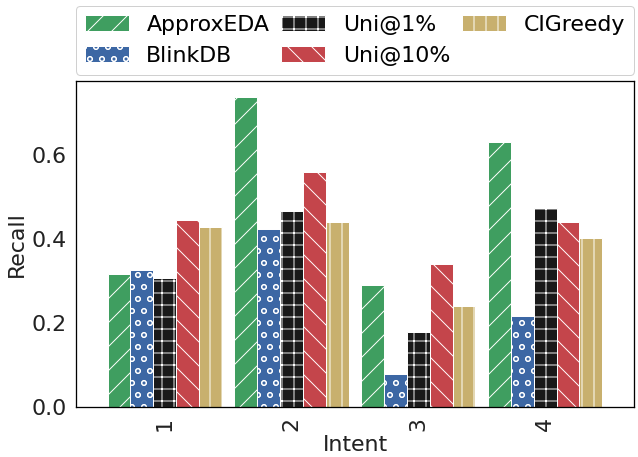
\includegraphics[width=1.0\linewidth]{LaTeX/figures/flights_eval1.png}
% \caption{Flights Dataset}
% \end{subfigure}
% \begin{subfigure}{0.5\textwidth}
% 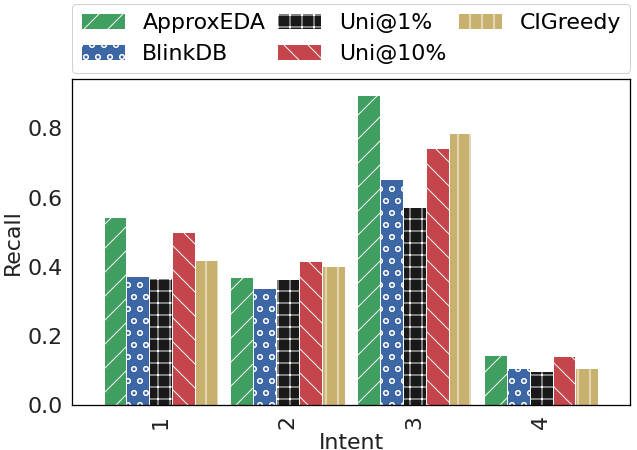
\includegraphics[width=1.0\linewidth]{LaTeX/figures/housing_eval1.png}
% \caption{Housing Dataset}
% \end{subfigure}
%      \caption{Insight Preservation: Recall of the resulting rows at the end of analysis sequence compared to results from full data, across various intents.
%      Higher is better.}
%      \label{fig:recall}
% \end{minipage}
% \end{figure*}


\subsection{Sampling Strategies}
\label{app:sampling_details}

A sample dataset $T_s$ is a subset of rows from an original dataset $T$. Following different sampling strategies select these subsets differently with different set of parameters that control the size and statistics of $T_s$.
%We now provide brief background for different sampling strategies we used. 

\noindent \textbf{Uniform Random Sampling:}
In uniform sampling, the rows of $T$ are
sampled independently (i.e, a Bernoulli process) with a sampling probability equal to $\tau \in [0,1] $. $\tau$ is called the sampling frequency and different values lead to different sizes for $T_s$.
%(and consequently different query latency).
%Total size of the sample:
%$|T_s| \approx \tau|T|$ (Note, Bernoulli process may not return exact number of rows as calculated using sampling probability).

\noindent \textbf{Systematic Sampling:}
In a systematic sample~\cite{lohr2019sampling}, a starting row of data is chosen using a random number. That row, and every $k$-th row thereafter, is chosen to be in $T_s$.
%With systematic sample thus $T_s$ consists of rows that are equally spaced in the data.
%Total size of the sample:
%$|T_s| = \floor*{{|T|}/{k}}$.
%If the rows are in random order, $T_s$ behaves much like an uniform random sample.
%However, systematic sampling does not necessarily give a representative sample when the rows are in some periodic or cyclical order. 
%Example, if male and female names alternate in a dataset, and $k$ is even, then
%$T_s$ will have either all men or all women data and can lead to wrong insights. 

\noindent \textbf{Stratified Sampling:}
Let for a column $C$ in data $T$, there are $G$ unique categories (i.e. strata). 
Stratified sample ensures that \textit{enough} rows are selected in $T_s$ for each unique values
%${v_1, \ldots , v_g}$ 
in $G$. 
%With $x$ denoting a row, let
%
%$T_i = \{x : x \in T \text{and $x$ takes values $v_i$ in column $C$}\}$

%Instead of doing such stratification for each column or all combination of columns,~\cite{agarwal2013blinkdb} proposed to use query column sets (QCS) that appear frequently as part of the filters (\texttt{WHERE}) and \texttt{GROUP BY} clauses in the query to reduce approximation error for ad-hoc queries.

%There are primarily two kinds of stratified samples used for query processing:
%\begin{itemize}
    %\item 
\noindent\textbf{Proportional stratified sample:} 
    In this case uniform samples $T_{i_{s}}$ are picked for each strata $T_{i}$ with a sampling probability of $\tau$.
    %Final sample $T_s = \bigcup\limits_{i=1}^{g} T_{i_{s}}$.
    %Different values of $\tau$ is selected to achieve approximation-latency trade-off.
    %Total size of the sample become: 
    
    %$|T_s| = \sum\limits_{i=1}^{g}{|T_{i_{s}}|} = \sum\limits_{i=1}^{g}{\tau|T_{i}|} $
    
    %\item 
\noindent\textbf{At most $K$ stratified sample:}
    In this case, for each strata, at most $K$ values are randomly selected to be included in $T_s$~\cite{agarwal2013blinkdb}.
    %Total size of the sample becomes: 
    
    %$|T_s| = \sum\limits_{i=1}^{g}\min(K, |T_{i}|)$
%\end{itemize}

\noindent \textbf{Cluster Sampling:}
The data is clustered into $k$  clusters,
%similar to stratified sampling, uniform 
samples are picked from each cluster with a sampling probability of $\tau$.
%Final sample $T_s = \bigcup\limits_{i=1}^{k} T_{i_{c}}$. %Total size of the sample becomes:

%$|T_s| = \sum\limits_{i=1}^{k}{|T_{i_{c}}|} = \sum\limits_{i=1}^{k}{\tau|T_{i}|} $
%Cluster has a superficial resemblance to strata: A cluster, like a stratum, is a
%grouping of the rows in $T$.
%However, when stratification generally increases precision when compared with simple random sampling, cluster sampling generally decreases it~\cite{lohr2019sampling}.

\noindent \textbf{Diversity sampling:} 
%Diversity sampling ensures that the algorithm picks out a diverse set of rows, $T_s$ from $T$. 
This targets that the sample picked out has different types of rows inside~\cite{diversity2017}. 
%Given a measure of diversity $div$, a set of rows $T$ having $|T|$ elements, and an integer $k$, $k < |T|$, we want to form a set $T_s$ containing $k$ elements of $T$, such that:
%
%$ T_s = \underset{T_s'  \subseteq T, |T_s'| = k}{\mathrm{argmax}}\, div(T_s') $
%
Diversity is defined by a distance function $d$, including: (i) \textbf{MaxMin Diversity:} 
    This maximises the minimum pairwise diversity between elements of $T_s$. 
    %We define the $div$ function as follows,
    %
    %$div(T_s') = \underset{i,j \in T_s', i \neq j}{\mathrm{min}}\, d(i,j) $
and (ii)  \textbf{MaxSum Diversity:}
    This maximises the average pairwise diversity between elements of $T_s$. 


Tables \ref{tab:flights_samples}, \ref{tab:housing_samples} and \ref{tab:income_samples} show the sampling strategies and corresponding parameters used, actual size of the samples ($|T_s|)$ and presents the Effective Sampling Rate (ESR) for each of the three datasets we used to evaluate. Lower the sample size, lower would be the query latency but at the cost of different magnitude of approximation errors depending on the actual sampling strategy. 

\begin{figure}[h]

    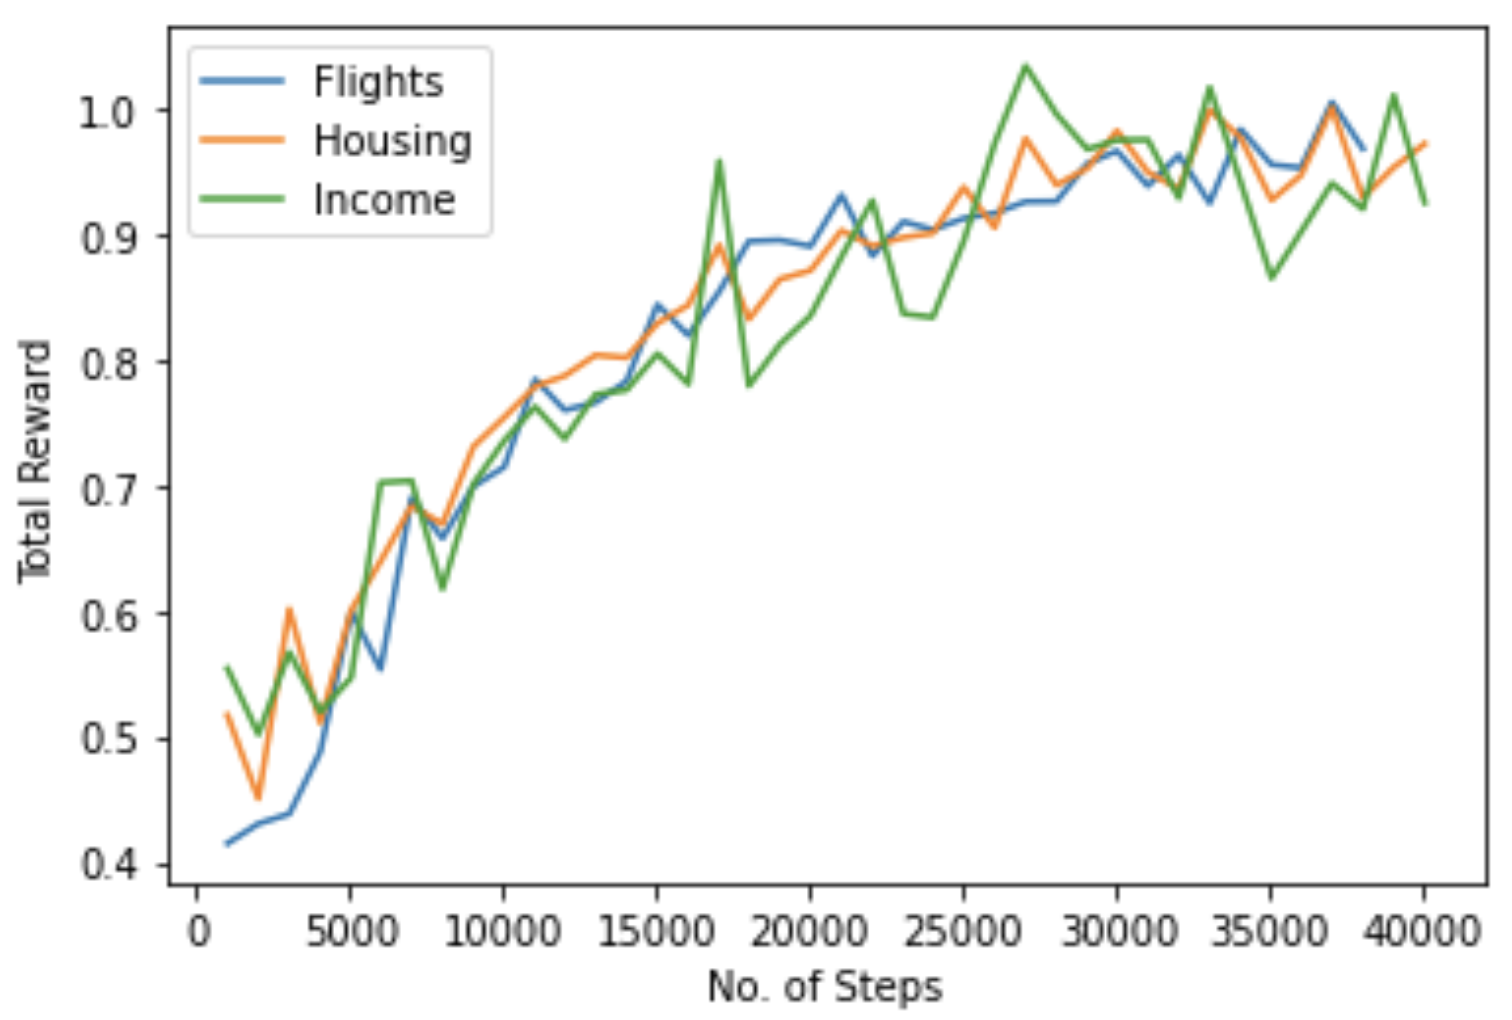
\includegraphics[width=1\linewidth]{LaTeX/figures/ss.png}
    \caption{RL training convergence curves for different datasets}
    \label{fig:my_conv}

\end{figure}
%\subsection{\name{} UI}
%
%In Figure~\ref{fig:demo} we show \name{}'s UI with which user will interact for EDA. The whole intelligence of \name{} remains almost transparent to the user. User can enable \name{} feature (blue box), to significantly improve interaction speed and \name{} will work at the background to choose optimal samples to run user-given query in an analysis flow and produce the results after each step. A log panel prints the actions taken by the RL-agent, along with corresponding query latency. Optionally, user can investigate the set of sampling strategies available. 